\chapter{Implementazione}
In questo capitolo viene descritta l'implementazione degli esperimenti
e vengono discusse le scelte implementative.
La prima sezione è dedicata agli strumenti utilizzati. Per prima cosa
viene introdotto PyTorch, il framework usato per 
definire le reti neurali usate, dopo viene introdotto Flower un 
framework per implementare e simulare sistemi di federated learning e 
per ultimo viene introdotto anche Hydra un tool per configurare 
molteplici esperimenti di datascience in python comodamente.

La seconda sezione invece è dedicata alle implementazioni fatte per 
questi esperimenti. In primis, viene indicato il codice utilizzato per 
caricare i dati dalle fonti menzionate nel capitolo precedente.
Successivamente vengono descritti i modelli usati per
i diversi esperimenti. Infine viene discussa l'ibridazione 
implementata dal modello di 
apprendimento federato a quello centralizzato, condividendo acluni 
sample dei dataset dei client in un unico dataset centralizzato.


\section{Gli strumenti}
\subsection{PyTorch}
PyTorch ~\cite{pytorch} è una libreria open-source estremamente popolare e flessibile 
per programmare ed allenare modelli di Deep Learning.
Siluppata inizialmente dal FAIR lab (Facebook's AI Reasearch), offre
un'API dichiarativa in python per costruire architetture di reti 
neurali, lasciando totale controllo al programmatore sul passo di 
feed forward di dati, facilitando la rapida sperimentazione di 
approci diversi e l'implementazione di pipeline
complesse come le GAN (Generative Adversarial Nets) ~\cite{goodfellow2014gan},
sperimentare tra transformer encoder-decoder ~\cite{vaswani2017trans}
o decoder only ~\cite{Radford2018ImprovingLU}.

PyTorch include una libreria estensiva di diversi tipi di layer,
loss functions, funzioni di attivazione e algoritmi di ottimizzazione
e la feature di autograd,
per cui facendo uso di un grafo dinamico di computazione PyTorch 
gestisce in automatico il calcolo del gradiente della loss function 
rispetto ad ogni parametro, rende l'implementazione di reti neurali 
estremamente facile, specie per casi particolarmente complicati 
come CNNs o RNNs.

\subsection{FlowerAI}
Flower (o FlowerAI) ~\cite{flowerai} è un framework open-soruce progettato semplificare
l'implementazione di sistemi di federated learning. Pur essendo una 
libreria python, supporta anche SDK per Android, iOS e C++, rendendolo 
ideale anche in ambienti mobile o di IoT.
Flower fornisce un'API per definire e implementare comodamente ogni 
specifico client in un apprendimento federato, configurandone il modello
da allenare, l'algoritmo di training e valutazione. Allo stesso modo è 
controllabile il comportamento del server e la strategia di aggregazione 
dei parametri aggiornati del modello forniti dai client  (i.e. un oggetto
di tipo flwr.server.strategy.Strategy).

Flower è stato usato per eseguire le simulazioni di apprendimento 
federato sui dataset FEMNIST e UCI HAR. In ogni simulazione, ogni client 
ha allenato il suo modello locale per un numero basso di epoche (5 per 
l'UCI HAR, 6 per il FEMNIST) e dopodiché manda i parametri aggiornati 
al server. La strategia utilizzata per aggregare i server è la
FedAvg. Questo ciclo  di allenamento e aggregazione 
costituisce un round ed ogni simulazione 
è durata 20 round.

Va notato che Flower è un framework pensato principalmente per il 
federated learning orizzontale e non ha un supporto nativo per 
contesti a partizionamento verticale. La soluzione, suggerita dallo 
stesso team di Flower ~\cite{flower_vfl}, è quella di riutilizzare 
il meccanismo di scambio di parametri da client a server per passare
invece l'encoding delle feature calcolato dal modello locale. 
L'effetto collaterale di questo sistema è che l'intero feed forward 
delle feature, nei modelli locali dei client ad encodings e poi 
nel modello del server da encoding a classificazione, richiede l'intero 
round di training. Questo implica che ogni round può eseguire una sola
epoca di training per round, cosa che può essere aggirata moltiplicando
il numero di round per il numero di epoche desiderate, e che si è
costretti ad un regime di full-batch training, a meno di non voler 
implementare una gestione delle batches dei dataset in funzione del 
round.

\subsection{Hydra}
Hydra ~\cite{hydra} è una libreria potente e flessibile per configurare 
ed eseguire molteplici esperimenti di data science implementati con 
script python. Le configurazioni in Hydra sono gestite tramite file 
\texttt{.yml}, ma permette anche la specifica di parametri dinamicamente
via command line. Supporta anche configurazioni gerarchiche, per cui 
è possibile specificare configurazioni di default da cui \textit{ereditare}
certi parametri e customizzarne altri per l'esperimento desiderato, in 
modo da permettere il riutilizzo delle configurazioni.

Supporta nativamente anche configurazioni "multi-run" per cui lo stesso 
script è eseguito più volte con configurazioni diverse, feature 
estremamente conveniente quando si vogliono provare diversi iperparametri
del proprio modello di machine learning, come in questo studio.

\section{Le implementazioni}

\subsection{Data loading}
\subsubsection{FEMNIST}
Come anticipato il FEMNIST è stato scaricato usando la repository di 
Xiao Chenguang ~\cite{femnist_hdf5}. Tale repository include uno script 
per generare due file, \texttt{write\_digits.hdf5} e \texttt{write\_all.hdf5},
per la versione dei dataset con e senza le immagini delle lettere.
Tale file, una volta letto, contiene un dizionario le cui chiavi sono 
id degli scrittori originali e gli elementi sono un'ulteriore dizionario 
con le due chiavi \texttt{"images"} e \texttt{"labels"} per i dati 
dell'immagine e il numero della rispettiva classe.

Quella che segue è la funzione
utilizzata per aprire il dataset \texttt{.hdf5} creato 
e istanziare i \texttt{Dataset} di PyTorch per ognuno dei client usati nella
simulazione:
\clearpage
\begin{lstlisting}
    def _get_femnist_datasets(
        num_writers: int,
        val_ratio: float,
        test_ratio: float,
        only_digits: bool = False,
    ) -> tuple[list[Dataset], list[Dataset], list[Dataset]]:    
        dataset_file = "write_digits.hdf5" if only_digits else "write_all.hdf5"
        full_dataset = h5py.File(f"data/{dataset_file}", "r")
        writers = sorted(full_dataset.keys())[:num_writers]
        train_sets = []
        val_sets = []
        test_sets = []
    
        for writer in writers:
            images = full_dataset[writer]["images"][:]
            labels = full_dataset[writer]["labels"][:]
            client_dataset = FemnistWriterDataset(
                images, labels, transform=femnist_transform
            )
    
            train_subset, val_subset, test_subset = _split_dataset(
                client_dataset, val_ratio, test_ratio
            )
            train_sets.append(train_subset)
            val_sets.append(val_subset)
            test_sets.append(test_subset)
    
        full_dataset.close()
        return train_sets, val_sets, test_sets
\end{lstlisting}
Tutti gli argomenti di questa funzione sono controllabili tramite la
configurazione Hydra usata per eseguire lo script. Si noti come
l'implementazione supporti anche un test di validazione per una 
possibile implementazione di early-stopping. I dataset di validazione 
sono però stati ignorati nel corso degli esperimenti e questa feature 
è rimasta da esperimenti preliminari.

\subsubsection{HAR}
Il dataset UCI HAR è distribuito direttamente dalla University of 
California Irvine~\cite{uci_har_ds}. Scaricato e decompresso il 
dataset, si possono trovare i dati separati nelle due cartelle 
\texttt{test} e \texttt{train}. Entrambe le cartelle contengono un 
file per le feature, un file per l'indice numerico della classe e un 
file con l'id della persona che ha compiuto l'azione. I sample sono 
scritti su questi file \texttt{.txt} riga per riga in modo 
corrispondente (la prima riga nel file di labels è la label per il 
feture vector nella prima riga del file di feature, che è stata 
compiuta dalla persona con id che compare nella prima riga). Per 
organizzare queste informazioni in \texttt{Dataset} PyTorch strutturato 
si è resa necessaria una funzione apposita che riassociasse le 
informazioni tra questi file.

Quelle che seguono sono le funzioni utilizzate per aprire i file del 
dataset come sono forniti dall'UCI i Dataset di PyTorch per 
ognuno dei client 30 e partizionare correttamente i sample:
\clearpage
\begin{lstlisting}
def _load_har_dataset(train: bool):
    variant = "train" if train else "test"
    full_features = [[] for _ in range(30)]
    full_labels = [[] for _ in range(30)]

    # get subject ids for measurements
    with open(f"data/subject_{variant}.txt", "r") as subject_file:
        subject_ids = [int(line.strip()) - 1 for line in subject_file]
    # get features and match them with the user
    with open(f"data/X_{variant}.txt", "r") as feature_file:
        for i, line in enumerate(feature_file):
            features = [float(num) for num in line.split()]
            full_features[subject_ids[i]].append(features)
    # get labels and match them with the user
    with open(f"data/y_{variant}.txt", "r") as label_file:
        for i, line in enumerate(label_file):
            label = int(line)
            one_hot = torch.zeros(6, dtype=torch.float32)
            one_hot[label - 1] = label
            full_labels[subject_ids[i]].append(one_hot)

    if train:
        return full_features, full_labels
    # flatten in one dataset for testing
    else:
        return [
            feature for user_features in full_features for feature in user_features
        ], [label for user_labels in full_labels for label in user_labels]


def _get_har_datasets() -> tuple[list[Dataset], Dataset]:
    train_features, train_labels = _load_har_dataset(True)
    test_features, test_labels = _load_har_dataset(False)

    client_datasets = [
        HarDataset(
            features=torch.tensor(train_features[cid], dtype=torch.float32),
            labels=train_labels[cid],
        )
        for cid in range(len(train_features))
        # some clients dont include measurements in the trainset
        if len(train_features[cid]) > 0
    ]
    test_dataset = HarDataset(
        torch.tensor(test_features, dtype=torch.float32), test_labels
    )
    return client_datasets, test_dataset
\end{lstlisting}

In questo caso la logica per istanziare il dataset federato è stata 
divisa in due funzioni in quanto, diversamente dal FEMNIST in cui il 
dataset originale è già partizionato per client, in questo caso c'è 
bisogno di (i) aprire 3 file diversi \texttt{subject\_\{variant\}.txt}, 
\texttt{X\_\{variant\}.txt} e \texttt{y\_\{variant\}.txt} e riassociare 
i dati tra loro e (ii) instanziare i \texttt{Dataset} di PyTorch.
La funzione \texttt{\_load\_har\_dataset} si occupa di fare la prima tasks,
mentre \texttt{\_get\_har\_datasets} si occupa di istanziare correttamente le classi 
\texttt{Dataset}. Si noti che i dataset locali sono partrizionati per 
utente, mentre il dataset di test è un unico dataset con sample di 
tutti gli utenti.


\subsection{I modelli}
Per tutti e 3 gli esperimenti condotti sono stati utilizzati modelli 
diversi.

\subsubsection{FEMNIST - CNN}
Per il dataset FEMNIST, essendo un problema di computer vision, è stata 
usata una CNN con 2 layer convoluzionali, rispettivamente con 32 e 
64 canali di output, con kernel size di 3, padding di 1
e max pooling tra di essi, seguiti da un layer fully connected 
di 512 neuroni. Il layer finale, di 10 o 62 neuroni a seconda che si 
usino le immagini delle sole cifre o di tutti i caratteri, usa una 
log softmax come funzione di attivazione, mentre tutti gli altri layer 
utilizzato la ReLU. L'implementazione in PyTorch di questa rete neurale
è la seguente:

\begin{lstlisting}
class CnnEmnist(nn.Module):
    def __init__(self, num_classes: int):
        super(CnnEmnist, self).__init__()
        # reused pooling layer
        self.pool = nn.MaxPool2d(kernel_size=2, stride=2, padding=0)
        # 2 convolutional layers
        self.conv1 = nn.Conv2d(
            in_channels=1,
            out_channels=32,
            ke
            \begin{figure}[htbp]  % h: here, t: top, b: bottom, p: page
                \centering
                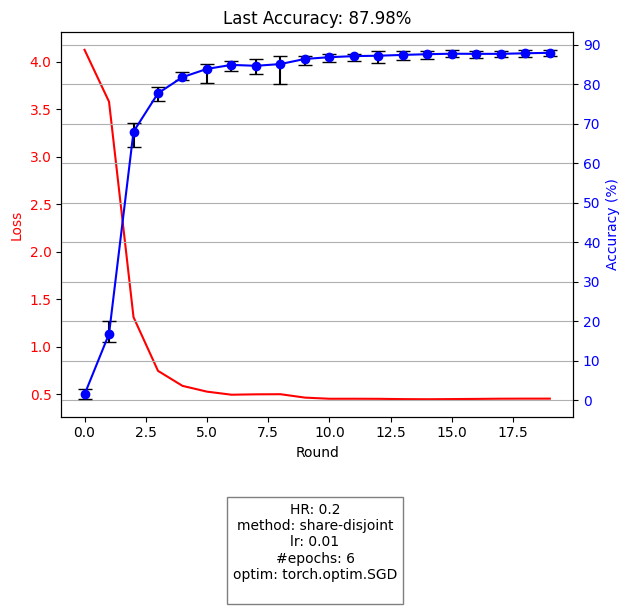
\includegraphics[width=0.8\textwidth]{../plots/femnist-horizontal/sgd/results-h0_2-hm_share-disjoint-lr0_01-e6-torch_optim_SGD.png}  % Adjust width as needed
                \caption{Caption describing the image}
                \label{fig:femnists2sgd}
            \end{figure}rnel_size=3,
            padding=1
        )
        self.conv2 = nn.Conv2d(
            in_channels=32,
            out_channels=64,
            kernel_size=3,
            padding=1,
        )
        # fully connected layer
        self.fc = nn.Linear(64 * 7 * 7, 512)
        # output layer
        self.classification = nn.Linear(512, num_classes)

    def forward(self, x):
        x = self.pool(F.relu(self.conv1(x)))
        x = self.pool(F.relu(self.conv2(x)))
        # flatten
        x = x.view(-1, 64 * 7 * 7)
        x = F.relu(self.fc(x))
        out = F.log_softmax(self.classification(x), dim=1)
        return out
\end{lstlisting}


\subsubsection{HAR HFL - MLP}
Il modello utilizzato per l'UCI HAR a partizionamento orizzontale 
è una semplice rete neurale composta di soli layer fully connected 
con un solo hidden layer. Ha un input per le 561 feature, un output 
di 6 neuroni per le 6 classi e un piccolo layer intermedio di 50 neuroni.
Nonostante le dimensioni ridotte del modello (28406 parametri totali)
si è riusciti comunque ad ottenere ottime prestazioni (> 90\%),
dimostrando la validità dell'approccio anche in contesti a risorse
ridotte, come telefoni o dispositivi IoT. Questa simulazione è stata 
anche eseguita interamente in CPU, senza accelerazione GPU, perché 
dato la maggiore quantità di RAM (32GB di RAM contro 6GB di VRAM
sulla GPU) sulla macchina usata per gli esperimenti, si è riusciti a 
terminare la simulazione più velocemente data la maggiore possibilità
di parallelizzazione del training svolto dai client. L'implementazione
di questo modello in PyTorch è la seguente:

\begin{lstlisting}
class HarModel(nn.Module):
    def __init__(self, num_classes: int):
        super(HarModel, self).__init__()
        self.fc1 = nn.Linear(561, 50)
        self.fc2 = nn.Linear(50, num_classes)

    def forward(self, x):
        x = F.relu(self.fc1(x))
        out = F.log_softmax(self.fc2(x), dim=1)
        return out
\end{lstlisting}


\subsubsection{HAR VFL - MLP distribuito}
In ultimo è stato anche provato un modello a partizionamento verticale 
delle feature dell'UCI HAR. In questo contesto, dati \(K\) client,
ogni modello di un client prende \(561/K\) feature e calcola un encoding 
di queste in un vettore dimensione \(d\). Le dimensioni del vettore 
provate sono state \(d=10\) e \(d=100\). Calcolati gli encodings, 
il server raccoglie \(K\) di questi encodings in unico vettore di lunghezza
\(Kd\). Questo vettore di encodings viene poi passato ad un ultima rete 
neurale fully connected con un layer nascosto di 50 neuroni e 
l'output è di nuovo un vettore di dimensione 6 per le 6 attività. Il 
modello dei client è stato implementato con il codice seguente:

\begin{lstlisting}
class ClientVerticalModel(nn.Module):
    def __init__(self, num_features: int):
        super(ClientVerticalModel, self).__init__()
        self.input = nn.Linear(num_features, 50)
        self.latent = nn.Linear(50, latent_vector_length)

    def forward(self, x):
        x = F.relu(self.input(x))
        latent = F.relu(self.latent(x))
        return latent
\end{lstlisting}

Mentre il codice per la rete del server che raccoglie gli encodings e 
calcola la classificazione dell'input è:

\begin{lstlisting}
class ServerVerticalModel(nn.Module):
    def __init__(self, num_clients, num_classes: int):
        super(ServerVerticalModel, self).__init__()
        self.input = nn.Linear(num_clients * latent_vector_length, 50)
        self.output = nn.Linear(50, num_classes)

    def forward(self, x):
        x = F.relu(self.input(x))
        out = F.log_softmax(self.output(x), dim=1)
        return out
\end{lstlisting}

Per comodità in fase di testing del modello è stato anche implementata 
una versione unica del modello, in grado di prendere le 561 feature e 
calcolare la classificazione direttamente, facendo uso dei modelli 
client e del modello server passati nel costruttore. Dato che può 
facilitare a comprendere meglio il funzionamento del VFL di seguito è
riportato anche il codice di questo modello:

\begin{lstlisting}
class FullVerticalModel(nn.Module):
    def __init__(
        self,
        client_models: list[ClientVerticalModel],
        server_model: ServerVerticalModel,
        num_clients: int,
    ):
        super(FullVerticalModel, self).__init__()
        self.client_models = client_models
        self.server_model = server_model
        self.num_clients = num_clients

    def forward(self, x):
        embeddings = []
        for cid, model in enumerate(self.client_models):
            extracted_features = extract_features(x, self.num_clients, cid)
            embeddings.append(model(extracted_features))

        embeddings_aggregated = torch.cat(embeddings, dim=1)
        return self.server_model(embeddings_aggregated)
\end{lstlisting}


Ognuno di questi modelli è stato allenato con Cross Entropy Loss
come loss function e con due diversi algoritmi di 
ottimizzazione.
Il primo provato è il classico SGC (Stochastic Gradient
Descent) con learning rate di 0.01 e momentum di 0.9. Esperimenti
preliminari hanno provato altri valori come un learning rate più basso
come 0.001 o più grande come 0.1 o la rimozione del momentum, ma le 
performance migliori sono state ottenute con i valori indicati 
precedentemente; la CNN per il FEMNIST non riusce nemmeno a convergere 
senza momentum e l'accuracy sul test dataset si ferma intorno al 6\%.
L'altro algoritmo usato è stato l'AdamW ~\cite{Loshchilov2017AdamW}, 
ovvero l'algoritmo Adam (Adaptive Movement Estimation) con weight 
decay. In esperimenti preliminari è anche stato provato l'Adam classico 
ma si è notato che sia il loss che la test accuracy erano molto 
instabili durante il training, suggerendo suggerendo che i parametri 
del modello fossero altrettanto instabili. Per tale motivo si è 
scelto di utilizzare la variante AdamW che implementa il weight decay 
come meccanismo di regolarizzazione per mantere i pesi del modello più
stabili. Si noti che si è evitato esplicitamente di utilizzare una 
L\sub{2} regularization come loss function per risolvere l'instabilità 
di Adam, dato che la L\sub{2} regularization e il weight decay sono 
equivalenti solo sotto SGD ~\cite{Loshchilov2017AdamW}.

\subsection{Ibridazione}
Per gli esperimenti a partizionamento orizzontale si sono fatti 
esperimenti per diversi gradi di ibridazione da simulazione completamente
federate a simulazioni completamente centralizzate. La configurazione 
dello script di training ammette due paramerti per controllare il grado 
di ibridazione da usare: \texttt{hybrid\_ratio} e 
\texttt{hybrid\_method}, che controllano
rispettivamente la percentuale dei dataset dei client da condividere in 
un unico dataset globale e il meccanismo di condivisione dei dataset.
Le tecniche di condivisione implementate sono state chiamate \texttt{unify}
e \texttt{share-disjoint}. Nel caso della \texttt{share-disjoint} ogni
client 
prende la percentuale indicata di sample dal suo dataset e li sposta
nel dataset condiviso, mentre nella \texttt{unify} la percentuale 
indicata di 
client condividono il loro dataset intero. Ad esempio, supponendo di 
avere 10 client con 10 dataset che contengono tutti 100 sample con un 
\texttt{hibrid\_ratio} di 0.2, con la \texttt{share-disjoint} ognuno 
dei 10 client prende
20 sample dal suo dataset e li mette nel dataset condiviso, ottenento 
un dataset condiviso di 200 sample e 10 client con 80 sample ciascuno,
mentre nella \text{unify} vengono selezionati randomicamente 2 client che 
condividono tutti i loro 100 sample, ottenendo un dataset condiviso di 
200 sampe e 8 client con 100 sample ciascuno.

Il codice che segue è il codice utilizzato per condividere parte dei 
dataset dei client, una volta che i dataset sono stati istanziati già
partizionanti per client:

\begin{lstlisting}
def _centralize_trainsets(
    train_sets: list[Dataset], num_clients: int, hybrid_ratio, hybrid_method
):
    if hybrid_method == "unify":
        num_centralized = int(hybrid_ratio * num_clients)
        shared_sets = []
        for _ in range(num_centralized):
            random_index = random.randint(0, len(train_sets) - 1)
            shared_sets.append(train_sets.pop(random_index))

        if num_centralized > 0:
            train_sets = [ConcatDataset(shared_sets)] + train_sets

    elif hybrid_method == "share-disjoint":
        # this method removes num_shared samples from clients and puts them in the collective
        shared_sets = []
        client_sets = []
        for train_set in train_sets:
            set_size = len(train_set)
            num_shared = int(hybrid_ratio * set_size)
            if num_shared > 0:
                shared_set, unshared_set = random_split(
                    train_set, [num_shared, set_size - num_shared]
                )
                shared_sets.append(shared_set)
                client_sets.append(unshared_set)
            else:
                # dont lose clients sets!
                client_sets.append(train_set)
        if len(shared_sets) > 0:
            train_sets = client_sets + [ConcatDataset(shared_sets)]

    return train_sets
\end{lstlisting}
